
Because in real life, it is difficult for athletes to precisely control the riding speed, let alone the output power. As a result, we need to consider the sensitivity of the model, especially the output power.
% Table generated by Excel2LaTeX from sheet 'Sheet1'
\begin{table}[h]
%		\renewcommand\arraystretch{0.9}
	\setlength\tabcolsep{13pt}%调列距
	\setlength{\belowcaptionskip}{0.2cm}
	\centering
	\caption{Strategies under different constraints for male}
	\begin{tabular}{ccc|cccc}
		\toprule[2pt]
		$P_1$    & $P_2$    & $P_3$    & $T_1$    & $T_2$    & $T_3$    & Total Time \\
		\midrule
		FTP   & 6.40  & 7.16  & 28:51 & 12:39 & 7:40  & 48:45 \\
		FTP   & \textbf{6.20 } & 6.76  & 28:51 & 6:58  & 13:14 & 49:04 \\
		FTP   & \textbf{6.00 } & 7.08  & 28:51 & 12:32 & 8:09  & 49:32 \\
		FTP   & 6.40  & \textbf{7.50 } & 28:51 & 15:04 & 4:51  & 48:46 \\
		FTP   & 6.40  & \textbf{8.00 } & 28:51 & 16:59 & 3:01  & 48:51 \\
		\bottomrule[2pt]
	\end{tabular}%
	\label{div}%
\end{table}%
\par In order to perform a sensitivity analysis, we change the parameter of power output for MTT, requiring the three stages of PO per kilogram to be constrained at a certain level. With new constraints, we get new results as table [\ref{div}].
% TODO: \usepackage{graphicx} required
\begin{figure}[h]
	\centering
	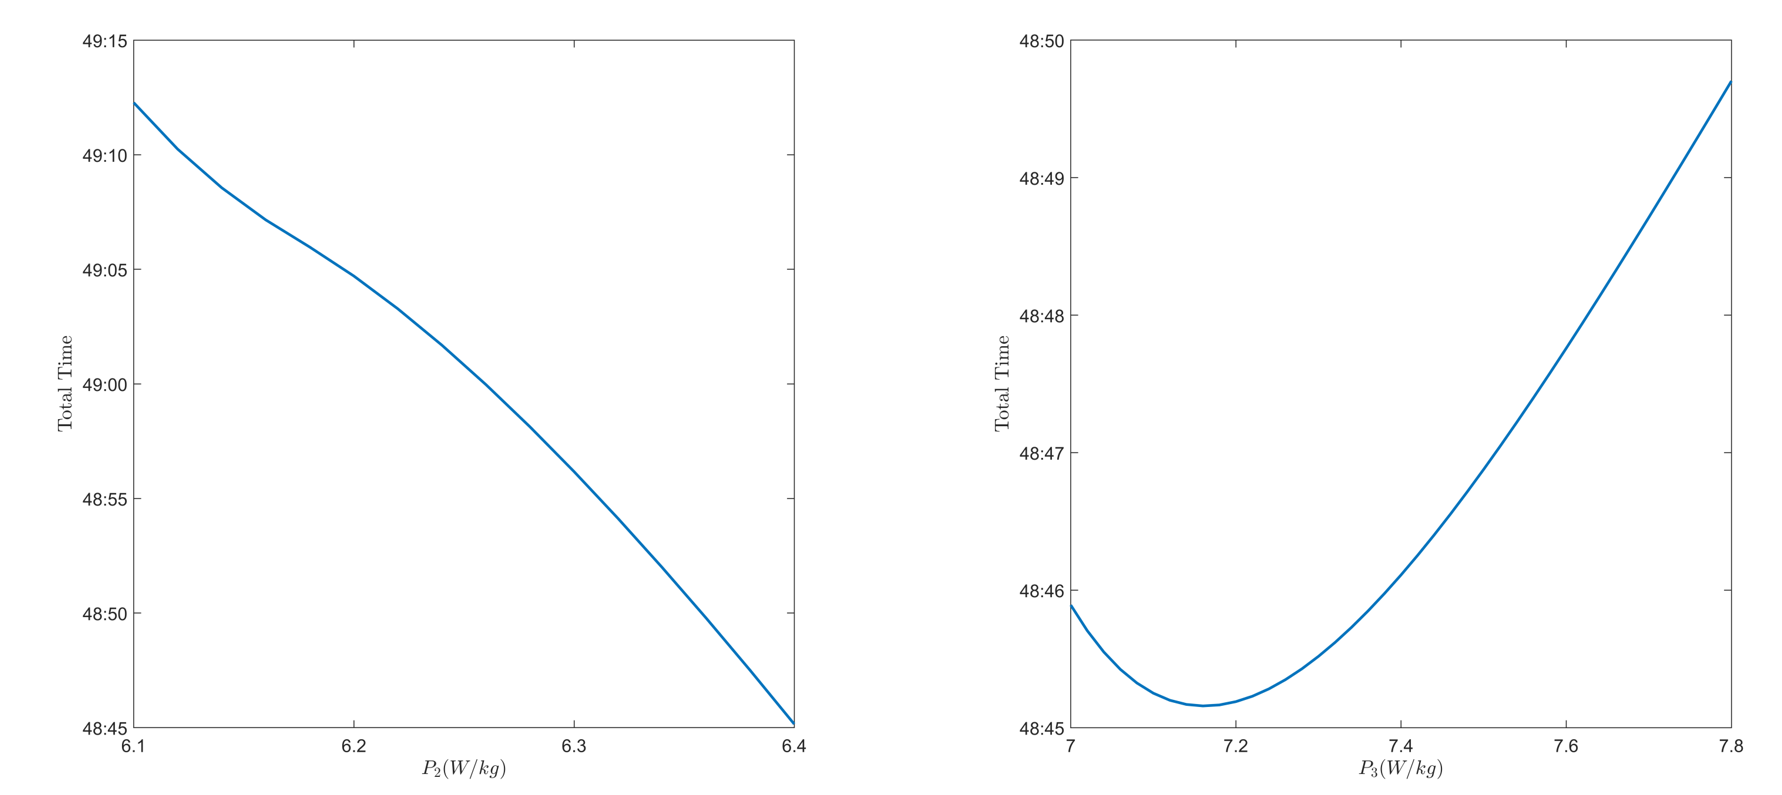
\includegraphics[width=0.7\linewidth]{image/p1}
	\caption{MTT Model sensitivity regarding $P_2$ and $P_3$}
	\label{P1}
\end{figure}
\par Through the same method, we obtain multiple sets of data and plotted the function between power output of two stages and total time for MTT [\ref{P1}]. 
\par As is shown in the curve, change in total time is always smaller as the output power changes at different stages, which shows that though riders does not have precise control over speed and power output, their score won't be much worse if follow our strategy. Also, the same method can be applied to the female virtual rider by changing the constraints and figuring out the optimal tactic, shown in table [\ref{time3}].
\begin{table}[h]
	%		\renewcommand\arraystretch{0.9}
	\setlength\tabcolsep{13pt}%调列距
	\setlength{\belowcaptionskip}{0.2cm}
	\centering
	\caption{Strategies under different constraints for female}
	\begin{tabular}{ccc|cccc}
		\toprule[2pt]
		$P_1$    & $P_2$    & $P_3$    & $T_1$    & $T_2$    & $T_3$    & Total Time \\
		\midrule
FTP   & 5.61  & 6.50  & 28:01 & 3:17  & 7:08  & 38:28 \\
FTP   & \textbf{5.50 } & 6.34  & 25:20 & 4:22  & 8:49  & 38:32 \\
FTP   & \textbf{5.40 } & 6.34  & 23:57 & 5:53  & 8:49  & 38:40 \\
FTP   & 5.61  & \textbf{6.60 } & 28:52 & 3:17  & 6:19  & 38:29 \\
FTP   & 5.61  & \textbf{6.70 } & 29:34 & 3:17  & 5:38  & 38:30 \\
	\bottomrule[2pt]
\end{tabular}%
\label{time3}%
\end{table}%
% TODO: \usepackage{graphicx} required
\begin{figure}[h]
	\centering
	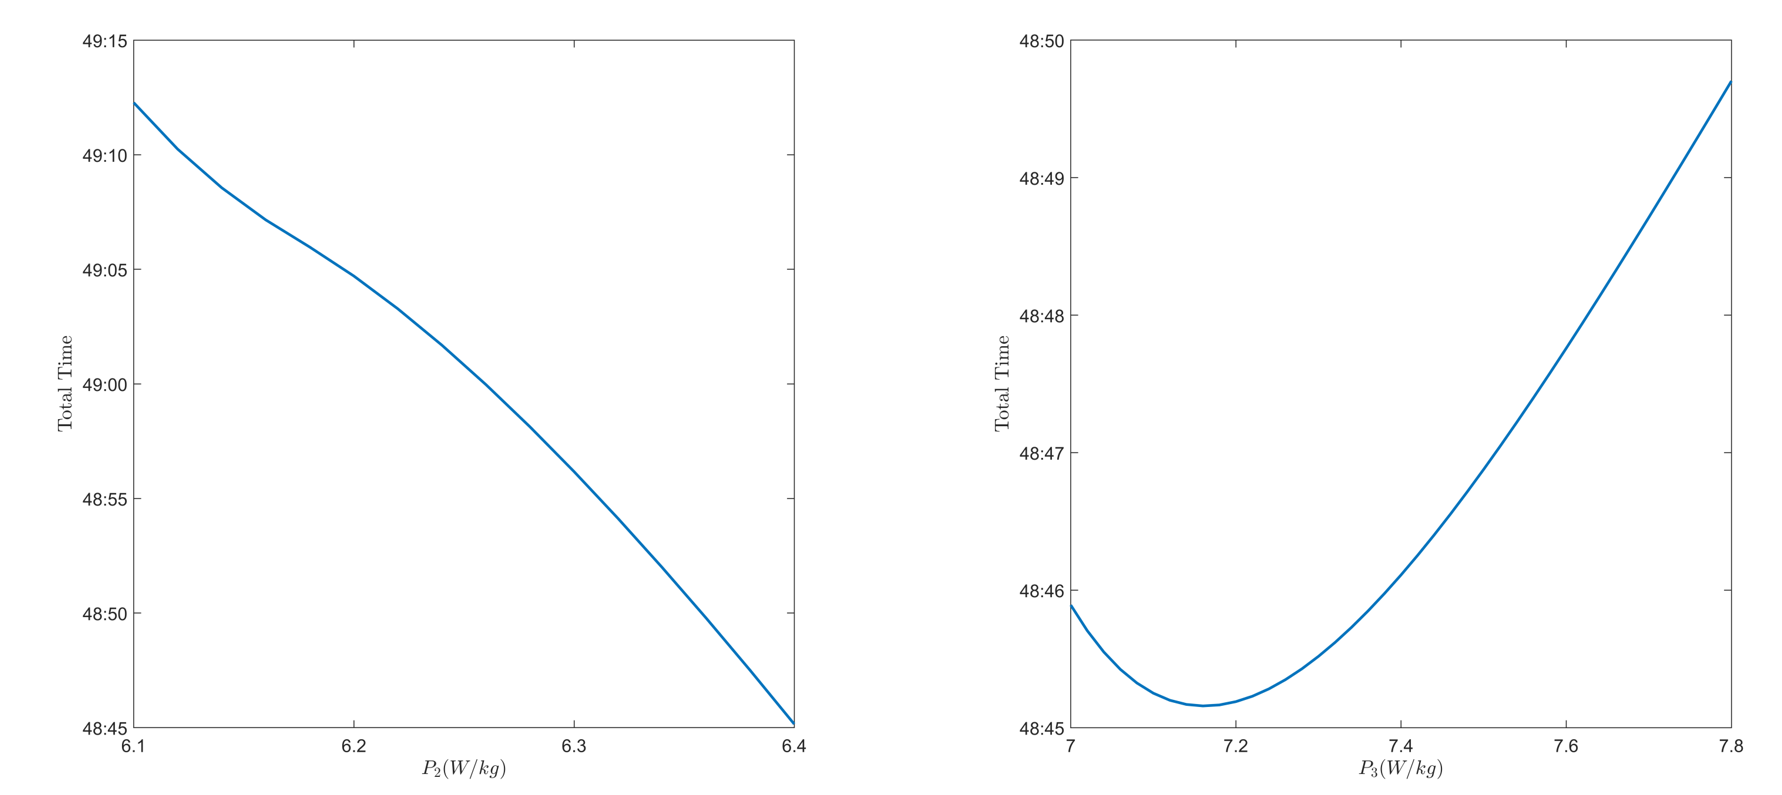
\includegraphics[width=0.7\linewidth]{image/p1}
	\caption{FTT Model sensitivity regarding $P_2$ and $P_3$}
	\label{P2}
\end{figure}

\par It can be inferred from the table that minor changes in power output won't cause significant difference in final scores(Total Time).Through the same method, multiple sets of data can be obtained by changing constraints, and the function is plotted between power output of two stages and total time  for FTT[\ref{P2}]. 
\par In conclusion, although our model can vary with output power, the change in total time is continuous with respect to the change in output power. Also, the change in total time is not significant with respect to variation in power output in different stages. As a result, it can be concluded that athletes can achieve ideal results within a power output range.

